\documentclass[a4paper, 11pt]{article}
\usepackage{comment} 
\usepackage{fullpage} 
\usepackage[spanish]{babel} 
\selectlanguage{spanish}
\usepackage[utf8]{inputenc}
\usepackage{float} 
\usepackage{graphicx}
\usepackage{ marvosym }
\usepackage{amsthm}
\usepackage{amsmath}
\usepackage[sort&compress, numbers]{natbib}
\usepackage{amssymb}
\usepackage{hyperref}
\hypersetup{colorlinks=True, citecolor=blue}


\begin{document}
\begin{center}
\LARGE \bf Pr\'actica 5\\ Método Monte-Carlo 
\end{center}

\vspace{1cm} 
\noindent\textbf {Edson Edgardo Samaniego Pantoja} \hfill \textbf{Materia:} Simulación computacional 
\hfill \\
\textbf{Fecha} \today  
\vspace{1cm} 

\section{Introducción}
El método Monte-Carlo proporciona soluciones aproximadas a una gran variedad de problemas matemáticos haciendo posible la realización de experimentos con muestreos de números pseudoaleatorios en una computadora es idóneo para situaciones en las cuales algún valor o alguna distribución no se conoce y resulta complicado de determinar de manera analítica.

\section{Metodología}
Se requiere aproximar el resultado de la siguiente integral:
\bigskip

$\int_3^7 \frac{dx}{\exp{(x)}+\exp{(-x)}}$
\bigskip

Se generan números pseudoaleatorios con distribución $g(x) = \frac{2f(x)}{\pi}$,  donde $f(x)= \frac{1}{\exp(x)+\exp(-x)}$.
Para la integral ya que se requiere el resultado para compararlo con lo que  se obtiene, se hace uso de la página WolframAlpha \cite{WA}, donde se ingresa la integral con sus límites y da un resultado de \texttt{0.048834}.
Para la práctica es utilizado un método de distribución de probabilidad que da solo valores positivos y todos estos juntos da uno, por decir representan un universo completo. Es dado un código en el repositorio de Schaeffer \cite{dra} donde se puede realizar el gráfico de distribución de probabilidad como el de la figura \ref{f1}, en el cual nosotros obtendremos la proporción dentro del intervalo de tres a siete, dentro del gráfico se genera un histograma de números pseudoaleatorios que siguen la función teórica analítica de $g(x)$.
\begin{figure}[H]
  \centering      
  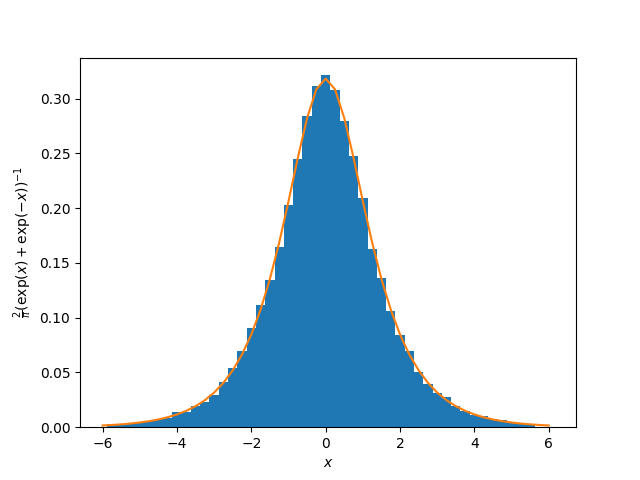
\includegraphics[scale=.7]{Figure_1.png}
  \caption{Gráfica de distribución de probabilidad e histograma de $g(x)$ \cite{Edson}.}
  \label{f1}
\end{figure}
\bigskip
Al tener la generación pseudoaleatoria se puede estimar la integral en el programa, utilizando como apoyo el código del repositorio de Schaeffer \cite{dra} el cual toma una muestra especificada dentro del intervalo de tres a siete, a partir de esto se saca un porcentaje de la cantidad que hay en el intervalo y la muestra tomada se sabrá el porcentaje que hay en esa fracción de valores con esto se renormaliza para recuperar el integral mediante funciones especificadas y nos retorna un valor parecido al obtenido en WolframAlpha.

\section{Objetivo}
El objetivo de la practica dado en la página de Schaeffer \cite{elisa}, es que con el código explicado anteriormente se pueda comparar el resultado de WolframAlpha de \texttt{0.048834} contra el resultado que arroja el programa. 
Más concreto y especifico se hará un análisis donde se comparará a partir de dos, tres, cuatro y cinco decimales realizando varias replicas para asegurar un porcentaje de eficiencia en cada decimal de precisión y en cada prueba con cada decimal se varia el número de muestras ya que esto afecta que tanta eficiencia hay conforme los decimales aumentan.
Lo importante es determinar el tamaño de muestra y representar el resultado como una sola gráfica con el número de decimales correctos contra el tamaño de muestra para una tasa de éxito que se elija.

\section{Simulación}
En el programa lo principal que se realiza es el cambio de decimales que para este caso se examinaran dos, tres y cuatro decimales, así que entrarán a un ciclo \texttt{for} que hará esta función, dentro del ciclo se asigna el valor de \texttt{n} en condiciones \texttt{if} de cada decimal y estas tienen su propio \texttt{n} que son el numero de muestras. El código completo puede ser consultado en el repositorio de Samaniego \cite{Edson}.
\bigskip
\begin{verbatim}
desde = 2.96
hasta = 7
replicas = 100

for decimales in (2, 3, 4):
    if decimales == 2:
        n=81000
    if decimales == 3:
        n=530000
    if decimales == 4:
        n=880000    
\end{verbatim}
\bigskip

Una vez que entra al primer ciclo con los primeros dos decimales y se le asigna el número de muestras, procede a otro ciclo \texttt{for} que es el generador pseudoaleatorio explicado anteriormente el cual da un resultado aproximado y variante dentro de la variable \texttt{numero}. Lo siguiente es como se comparan los decimales del valor recibido y el valor fijo nombrados \texttt{valor1} y \texttt{valor2} respectivamente, el método fue convertir los valores a \texttt{string} para de esta manera lograr separar cada dígito sólo que esta en formato de cadena así que después de tener los dos valores se procede a un ciclo que toma valor de la cantidad de decimales a leer y dentro los dos valores son convertidos a valores numéricos enteros (no cadena) para compararlos dato por dato y almacenarlo para después tomar una decisión donde si detecta un valor que es distinto dentro de los decimales comparados, este sumara un entero a la variable \texttt{similar} y al final tener la suma de cuantas veces no coincidió el número pseudoaleatorio con el valor fijo.

\begin{verbatim}
    for C in range(replicas):
        generador = GeneralRandom(np.asarray(X), np.asarray(Y))
        V = generador.random(n)[0]
        mc = ((V >= desde) & (V <= hasta))
        numero=((pi / 2) * integral)
        valor1= 0.048834
        valor2= numero
        for x in str(valor1):
            digito1.append(x)          
        for y in str(valor2):
            digito2.append(y)           
        for z in range(decimales):
            A=(int(digito1[z+2])==int(digito2[z+2]))
            comparacion.append(A)    
        if all(s==True for s in comparacion)== False:
            similar.append(1)
\end{verbatim}

\bigskip

Una vez acumulado cuantas replicas difirieron se procede a sacar el porcentaje de efectividad utilizando una regla de tres donde a las \texttt{replicas} realizadas se le esta restando la acumulación de diferencias por cien y dividido entre el total de \texttt{replicas}.

 \bigskip
 
\begin{verbatim}
         cuantos=(len(similar))
         porcentaje = (((replicas-cuantos)*100)/(replicas))
         print(porcentaje,'%')
\end{verbatim}

\section{Ajustes de programa}
Este apartado consta de cambios en la programación base donde se produce la integral y sus límites, debido a qué con dichos rangos de tres a siete se hacen pruebas con un número de muestras alto de hasta quinientos mil y se muestra que el resultado no pasa la condición de más de dos decimales coincidentes a el valor fijo de \texttt{0.048834}, por lo que se opta por ampliar los límites para un mayor intervalo de muestras quedando de 2.96 a siete, así es como hubo una mejora y un mayor porcentaje de coincidencia en tres decimales. 
Otro cambio realizado en el programa o más bien una decisión que se tomo es no utilizar cinco decimales debido a que el número de muestras era excesivamente alto y la computadora tardaría mucho tiempo en procesar las cien replicas y el porcentaje de efectividad sería muy bajo.

\section{Resultados}
Las pruebas se realizaron en repetidas ocasiones para poder obtener los resultados mas estables a una tasa de éxito fija de cada decimal por ejemplo para dos decimales se fijo la tasa a \texttt{90\%} con una cantidad de ochenta y un mil muestras que se puede observar en el cuadro \ref{tab1}. 
    \begin{table}[H]
        \caption{Registro de muestras por cada decimal de precisión, número de replicas realizadas en la prueba y el porcentaje de efectividad obtenido del total de replicas.}
        \bigskip
        \label{tab1}
        \centering
        \begin{tabular}{|r|r|r|r|}
        \hline
         Decimales&Muestras&Replicas&Porcentaje de efectividad  \\
        \hline
        2 & 81000 & 100 & 90\%  \\
        \hline
        3 & 530000  & 100 & 80\%  \\
        \hline
        4 & 880000  & 100 & 10\% \\
        \hline
        \end{tabular}
    \end{table}
\bigskip

Para mejor representación de los datos tabulados se realiza un gráfico de puntos de cada decimal de precisión y la cantidad de muestras realizadas para su tasa de efectividad \ref{f3} y adjunto a esto una línea que muestra el cambio o incremento de muestras conforme se busca más precisión por decimal, se puede observar que el cambio de dos a tres decimales implicó un aumento de muestras de \texttt{$449000$} aunque el porcentaje sólo se estableció de \texttt{80\%} debido a la tardanza de la obtención de datos, y para los cuatro decimales el porcentaje fue mas bajo de \texttt{10\%} debido a que las muestras fueron muy altas \texttt{$880000$} obteniendo una diferencia de muestras de \texttt{$350000$} entre tres y cuatro decimales.
\begin{figure}[H]
  \centering      
  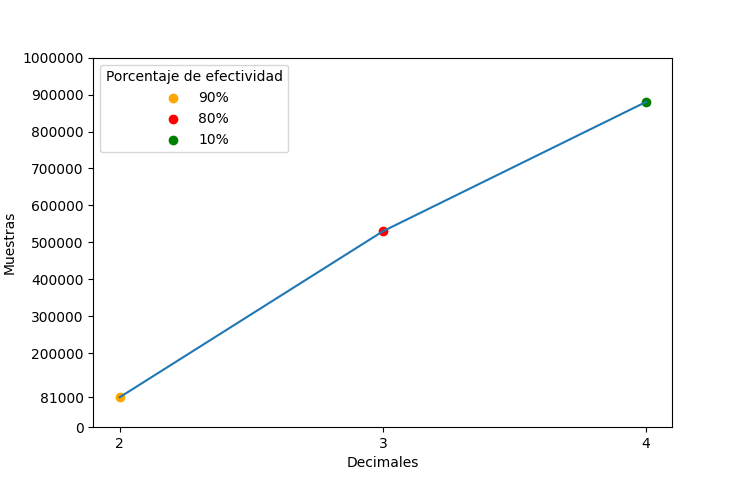
\includegraphics[scale=.7]{Figu.png}
  \caption{Gráfica de cantidad de muestras por decimal de precisión y tasa de éxito.}
  \label{f3}
\end{figure}

\bigskip

Por último se representa en un diagrama caja-bigote \ref{f2} de cada decimal como fueron sus replicas en lo que respecta a su distribución y se puede observar que conforme aumentaban los decimales de precisión, el número ya no era tan disperso ya que se acercaba más al valor obtenido en WolframAlpha pero vemos que en promedio la mayor cantidad de datos se mantuvo en el rango de \texttt{0.048} y \texttt{0.049}.
\begin{figure}[H]
  \centering      
  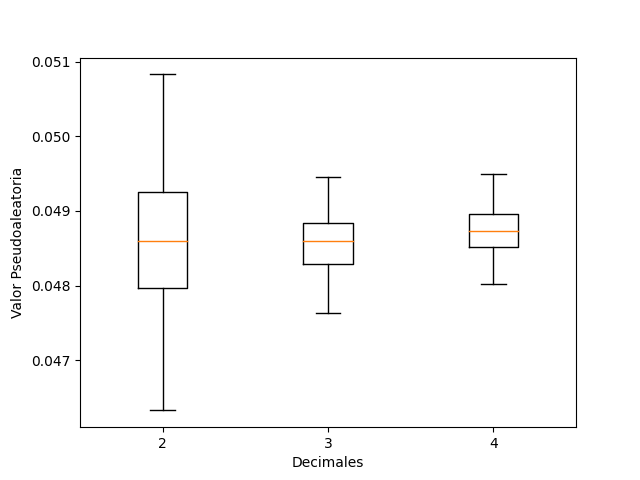
\includegraphics[scale=.7]{Figure_2.png}
  \caption{Caja-bigote por cada decimal y su distribución de replicas de valor pseudoaleatorio.}
  \label{f2}
\end{figure}
\bigskip
\bigskip

\bibliography{refe}
\bibliographystyle{plainnat}




\end{document}